\documentclass[12pt]{article}
 \usepackage[margin=2cm, bottom=3cm, top=2cm]{geometry}
% \usepackage[margin=1.0in]{geometry}
% \usepackage{textpos}
% \everymath{\displaystyle}
\newcommand{\vs}{\vspace{18pt}}

\usepackage{amsmath,amsfonts,amsthm,amssymb}
\usepackage{extramarks}
\usepackage{fancyhdr}
\usepackage{ifthen}
\usepackage{enumitem}
\usepackage{graphicx}
\pagestyle{fancy}

\pagenumbering{gobble}
\setlength\parindent{0pt}
%
% Create Problem Sections
%
\newcommand{\enterProblemHeader}[1]{
\nobreak\extramarks{}{Problem \arabic{#1} continued on next page\ldots}\nobreak\
{}
\nobreak\extramarks{Problem \arabic{#1} (continued)}{Problem \arabic{#1} contin\
ued on next page\ldots}\nobreak{}
}
\newcommand{\exitProblemHeader}[1]{
\nobreak\extramarks{Problem \arabic{#1} (continued)}{Problem \arabic{#1} contin\
ued on next page\ldots}\nobreak{}
\stepcounter{#1}
\nobreak\extramarks{Problem \arabic{#1}}{}\nobreak{}
}

\setcounter{secnumdepth}{0}
\newcounter{partCounter}
\newcounter{homeworkProblemCounter}
\setcounter{homeworkProblemCounter}{1}
\nobreak\extramarks{Problem \arabic{homeworkProblemCounter}}{}\nobreak{}
%
% Homework Problem Environment
%
% This environment takes an optional argument. When given, it will
% adjust the
% problem counter. This is useful for when the problems given for your
% assignment aren't sequential. See the last 3 problems of this
% template for an
% example.
%                                                          ~%
%
% Homework Problem Environment
%
% This environment takes an optional argument. When given, it will adjust the
% problem counter. This is useful for when the problems given for your
% assignment aren't sequential. See the last 3 problems of this template for an
% example.
%

\newenvironment{homeworkProblem}[1][-1]{
\ifnum#1>0
\setcounter{homeworkProblemCounter}{#1}
\fi
\subsubsection{Problem \arabic{homeworkProblemCounter}}
\setcounter{partCounter}{1}
\enterProblemHeader{homeworkProblemCounter}
}{
  \vspace{35ex}
  \exitProblemHeader{homeworkProblemCounter}
}
\newcommand{\footer}{
\rfoot{\ifthenelse{\value{page}=1}{\textbf{This quiz has 2 sides}}{}}
}
\newcommand{\header}{
\lhead{\large MATH 1210}
\chead{\large Implicit Differentiation \& 1st Deriv
  Applications Quiz} 
\rhead{\large Fall 2017}
{{Name and computing ID:} \underline{\hspace{3in}}}\\ \ \\
\fbox{
\begin{minipage}{6.5 in}
\textit{On my honor as a student, I pledge that I have neither given nor received help on this assignment.} \\ \ \\
{Signature:} {\underline {\hspace{3in}}}
\end{minipage}}
}

\everymath{\displaystyle}

%%%%%%%%%%%%%%%%%%%%%%%%%%%%%%%%%%%%%%%%%%%%%
\author{Math 1210}
\title{(More Challenging) Related Rates Practice Problems}

\begin{document}
\maketitle
% \begin{textblock*}{100mm}(.65\textwidth,-5.3cm)
%   Name:\underline{\qquad\qquad\qquad\qquad\qquad\qquad}
% \end{textblock*}
%%%%%%%%%%%%%%%%%%%%%%%%%%%%%%%%%%%%%%%%%%%%%
\begin{homeworkProblem}
  Water flows from a tank of constant cross-sectional area \(50\)
  ft\({}^2\) through an orifice of constant cross-sectional area
  \(1.4\) ft\({}^2\) located at the bottom of the tank (see the
  figure). Initially the height of the water in the tank was \(20\)
  ft, and its height \(t\) sec later is given by the equation \[
    2 \sqrt{h} + \frac{1}{25}t - 2 \sqrt{20} = 0 \hspace{1in} (0 \leq
    t \leq 50 \sqrt{20})
  \]
  How fast was the height of the water decreasing when its height was
  \(8\) ft? \\
  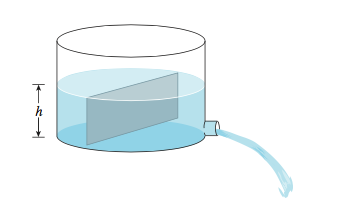
\includegraphics[scale=0.5]{images/water-tank}
\end{homeworkProblem}
\begin{homeworkProblem}
  A water trough is \(10\) m long and a cross-section has the shape of
  an icosceles trapezoid that is \(30\) cm wide at the bottom, \(80\)
  cm wide at the top, and has height \(50\) cm. If the trough is being
  filled with water at the rate of \(0.2\) m\({}^3\)/min, how fast is
  the water level rising when the water is \(30\) cm deep.
\end{homeworkProblem}
\begin{homeworkProblem}
  If two resistors with resistances \(R_1\) and \(R_2\) are connected
  in parallel, as in the figure, then the total resistance \(R\),
  measured in ohms (\(\Omega\)), is given by \[
    \frac{1}{R} = \frac{1}{R_1} + \frac{1}{R_2}
  \]
  If \(R_1\) and \(R_2\) are increasing at rates \(0.3 \Omega/\)s and
  \(0.2 \Omega/\)s, respectively, how fast is \(R\) changing when
  \(R_1 = 80 \Omega\) and \(R_2 = 100 \Omega\)? \\
  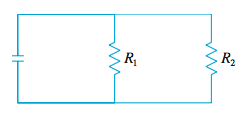
\includegraphics[scale=0.5]{images/resistors} 
\end{homeworkProblem}
\begin{homeworkProblem}
  Boyle's Law states that when a sample of gas is compressed at a
  constant temperature, the pressure \(P\) and volume \(V\) satisfy
  the equation \(PV=C\), where \(C\) is a constant. Suppose that at a
  certain instant the volume is \(600\) cm\({}^3\), the pressure is
  \(150\) kPa/min. At what rate is the volume decreasing at this instant?
\end{homeworkProblem}
\end{document}